\documentclass[journal]{IEEEtran}

% Package to commnet out sections.
\usepackage{comment} 

% Package to make referenzes become ``hyperlinks''
\usepackage{hyperref}

% Package for drawings.
\usepackage{tikz}
\usepackage{caption}
\usepackage{subcaption}

% Get the encoding and language right.
\usepackage[utf8]{inputenc}
% \usepackage[ngerman]{babel}

\usepackage{graphicx}                  % This is needed for including figures and graphics
\usepackage{amssymb}
\usepackage{epstopdf}
\DeclareGraphicsRule{.tif}{png}{.png}{`convert #1 `dirname #1`/`basename #1 .tif`.png}

\title{VP Bericht - Elektronik D}
\author{Julian Viereck}
\date{\today}                                           % Activate to display a given date or no date

\begin{document}

\maketitle

\begin{abstract}
\end{abstract}

\tableofcontents

\section{Introduction}

In this experiment, some of the basic concepts of digital circuits are explored.
Digital circuits contain logic gate. The gates transform a
digital input signal into some digital output signal following a well defined functionality.
The input and output signal are either ``high/1'' or ``low/0''. This is a main
difference compared to the analogous circuits, which have a continuous range of
input/output signals. In today's world gates play an important role in. Every
digital circuit contains a few up to multiple billions of them.

TODO: Write something about IC.

Gates can be categorized by gate-family, that they belong to (e.g. TTL or CMOS)
and some other specific properties. Gates perform different operations to
``compute'' the output signal based on some input signal. Also, gates differ in
terms of propagation delay, which is the delay a change in one of the input
signals takes to cause a change in the output signal. The propagation delay is
very important when designing digital circuits.

In the following, the performed experiments are presented. The experiments
describe how to determine the operation performed by a digital circuit and it's
propagation delay, how a pulse generator is build and how to implement a very
simple bit shifter logic.

\section{Experiment simple logic gate}

\subsection{Samples and measurement setup}

\begin{figure}[h!]
  \centering
   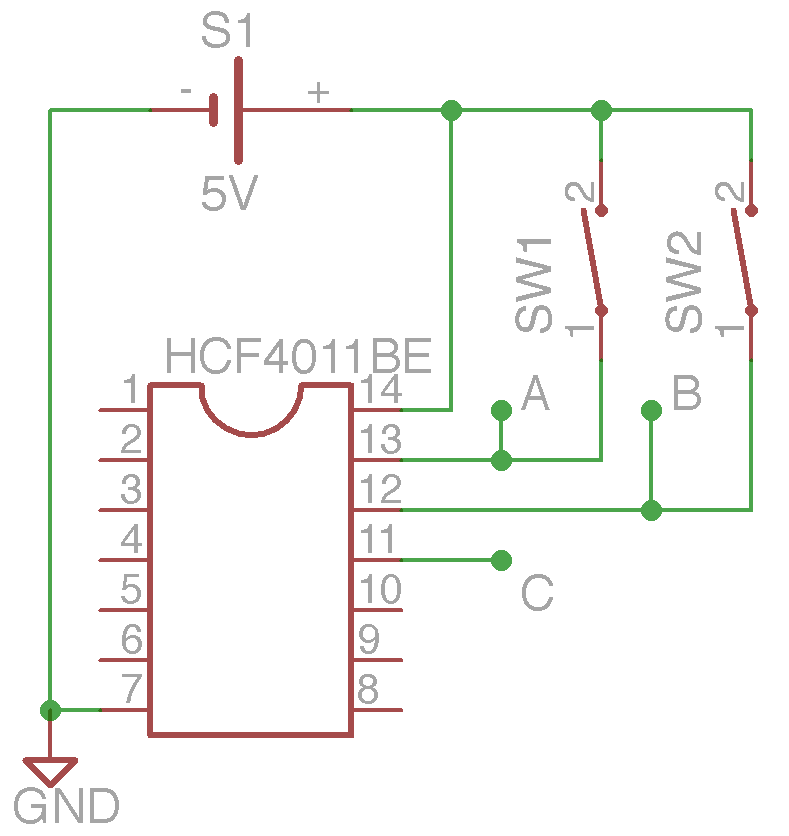
\includegraphics[]{boards/truth.png}
   \caption{Circuit diagram to measure truth table.}
   \label{fig:truth_circuit}
\end{figure}

The circuit was setup as shown in figure \ref{fig:truth_circuit}. Based on the
different input signals at A and B, different values for the output signal C
were measured using a oscilloscope. As for the ICs, a HCF4001BE and HCF4011BE
were used.

To measure the propagation delay, input signal A was connect to a square wave
voltage generator. Input signal B was connected to ground. The IC HCF4001BE
was used for this measurement. The voltage of the generator was set to 2.9V and
the frequency to 1Hz. The input signal A and output signal C was visualized
using a oscilloscope. The oscilloscope's trigger signal was connected to the voltage
generator.

\subsection{Results}

\begin{figure}
	\centering
	\begin{tabular}{c c | c || c c | c}
 		 \multicolumn{2}{c}{4011}
  		 \multicolumn{5}{c}{4001} \\
		  A & B & C & A & B & C \\ \hline
		  0 & 0 & 1 & 0 & 0 & 1 \\
		  0 & 1 & 1 & 0 & 1 & 0 \\
		  1 & 0 & 1 & 1 & 0 & 0 \\
		  1 & 1 & 0 & 1 & 1 & 0 \\
	\end{tabular}
	\caption{Truth table measuring IC HCF40011BE and HCF4001BE}
	\label{tab:truthtable} 
\end{figure}

 \begin{figure}
   \centering
  \begin{tikzpicture}
    \node[anchor=south west,inner sep=0] at (0,0)
    {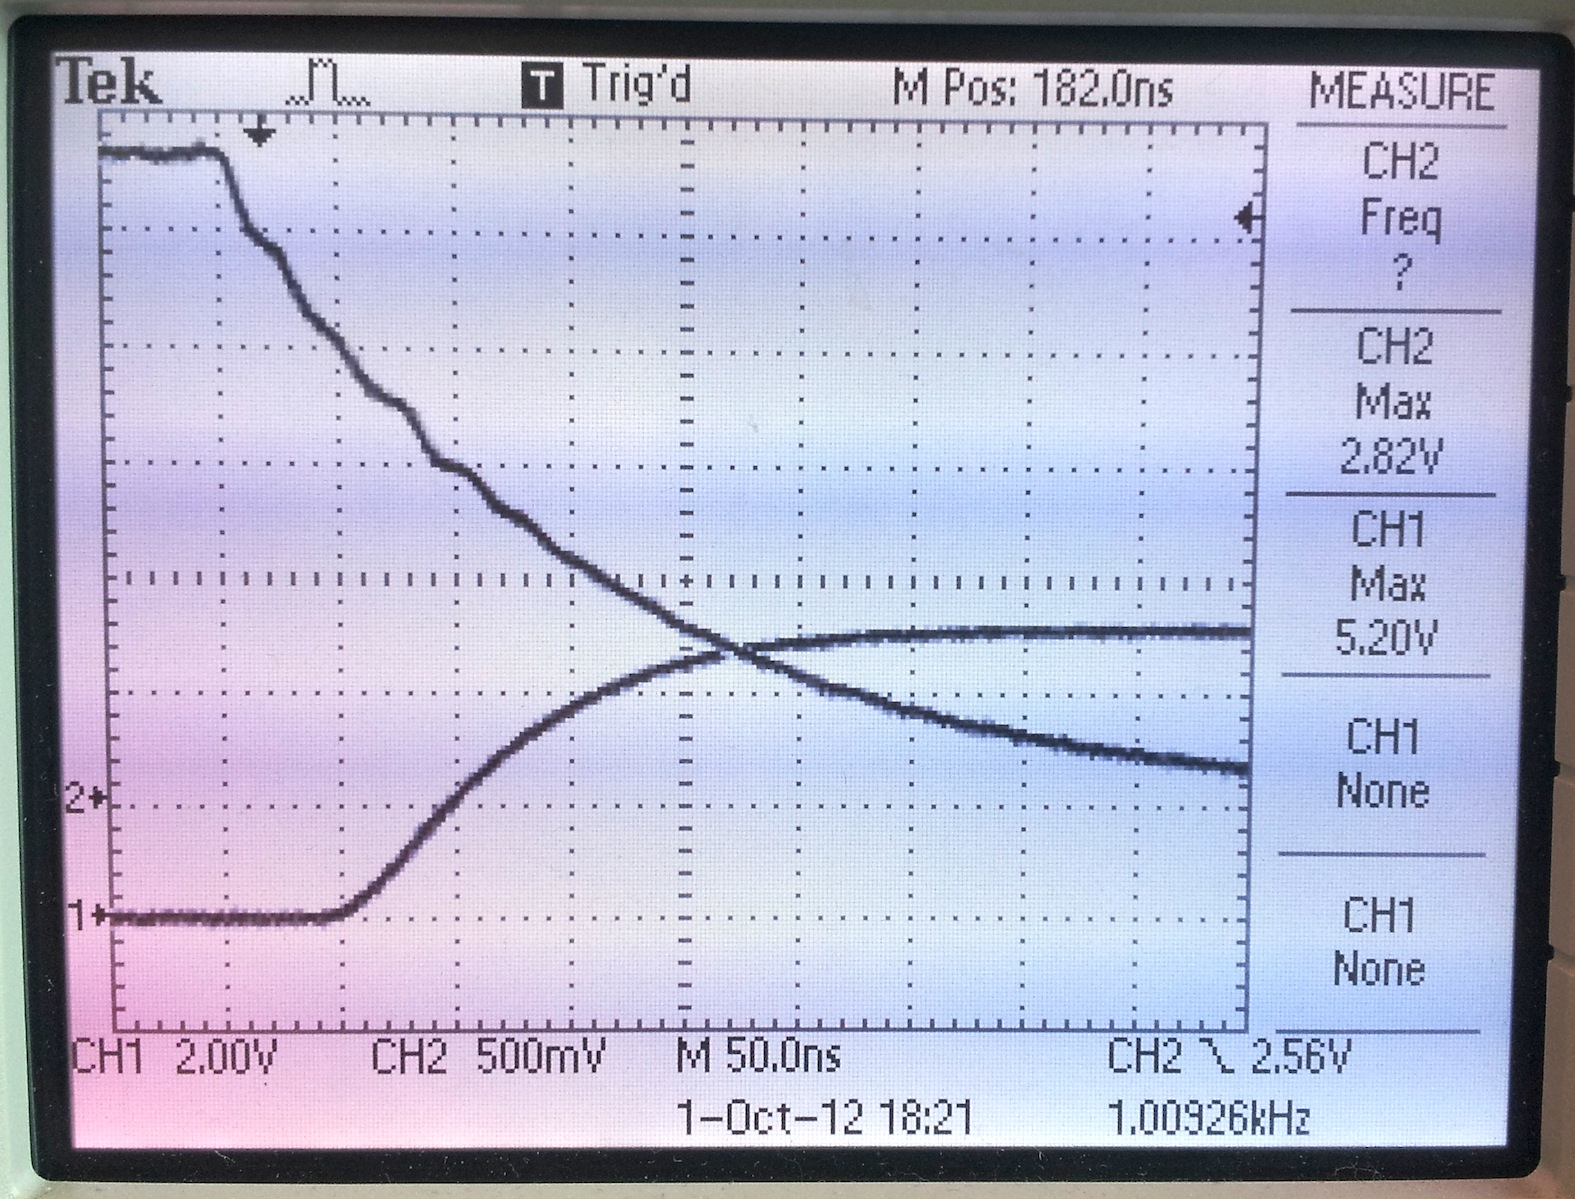
\includegraphics[width=\columnwidth]{img/delay.jpg}};
    \draw[color=red] (1.2,1.1) -- (1.2,6);
    \draw[color=red] (1.9,1.1) -- (1.9,6);
    \path[<->] (1.2, 3) edge node[below]{$\approx 50ns$} (1.9,3);
    \path[<-] (3.3, 3.8) edge node[near end, align=left, right]{Input signal A}
    (4,5);
    \path[<-] (3.3, 2.5) edge node[near end, align=left, right]{Output signal C}
    (4,1.2);
  \end{tikzpicture}
  \caption{Propagation delay measurement.}
  \label{fig:propdelay}
\end{figure}

For different input signals A and B, the truth-table was measured as
shown in table \ref{tab:truthtable}.

The propagation delay was measured to be around 50ns as seen in figure
\ref{fig:propdelay}.

\subsection{Analysis and Discussion}

Based on the measurements, the IC HCF4001BE seems to be a logic NOR gate,
whereas the IC HCF4011BE seems to function as a NAND gate. This fits with the
specified functionality of the gates.

Looking up the propagation delay from the data sheet, it is said to be typically
around 40ns and up to 75ns. This fits with the here measured delay.

\section{Pulse Generator}

A pulse generators are used to create rectangular, periodic voltage signals. In
this experiment, such a generator was build and its properties examined. 

\subsection{Samples and measurement setup}

\begin{figure}[h!]
  \centering
   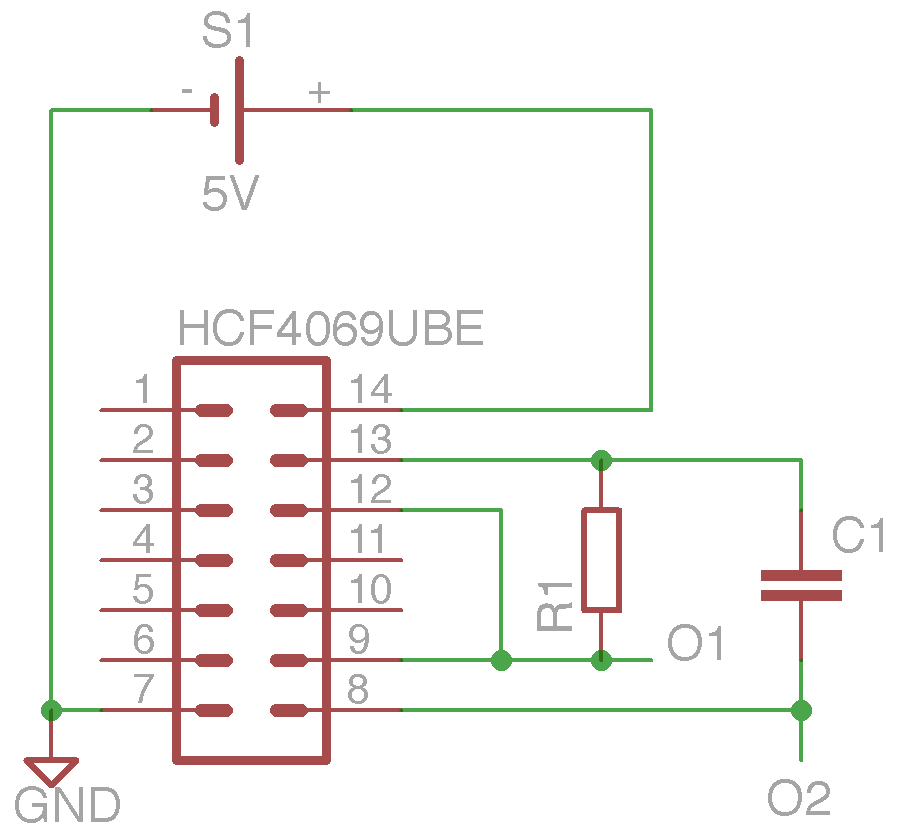
\includegraphics[]{boards/astabil_multivibrator.png}
   \caption{Circuit diagram of astable multivibrator.}
   \label{fig:am_board}
\end{figure}

The circuit was assembled as shown in figure \ref{fig:am_board}. Here, the IC
HCF4069UBE was used, which contains six NOT gates. The voltage difference
between the output signals $O1$, $O2$ and the ground was quantified using an
oscilloscope. This also allowed to visualize and measure the period of the
oscillations.
Different values for the resistance $R1$ and the capacity $C1$ were chosen and
the resulting period of the voltage signals determined.

\subsection{Functionality explanation}

\begin{figure}[h!]
  \centering
   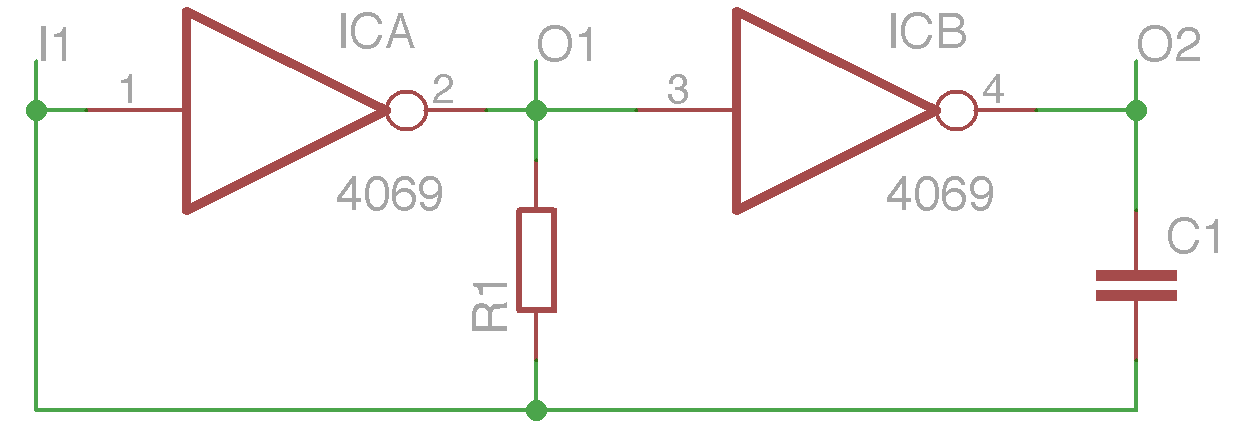
\includegraphics[]{boards/am_overview.png}
   \caption{schematic drawing of the astable multivibrator circuit.}
   \label{fig:am_scheme}
\end{figure}

A schematic drawing of the circuit is presented in figure \ref{fig:am_scheme}.
The explanation follows the one given in \cite{book_dg}. Let's assume the
voltage at $O1$ is set to be \emph{high} and the capacitor is uncharged. Due to
the \emph{high} signal at $O1$, the signal at $O2$ is \emph{low}. Over the
resistance $R1$ the capacitor is charged. At some point, the voltage at $I1$ is high enough, such
that the input signal of $ICA$ is recognized as \emph{high}. This causes the
signal at $O1$ to become \emph{low} and therefore the signal at $O2$ to be
\emph{high}. The charged capacitor discharges, which keeps the \emph{high}
signal at the $I1$ input for some time until the voltage on the capacitor is to
low, such that the signal at $I1$ is recognized as a \emph{low} signal, the
signal at $O1$ becomes a \emph{high} one and things start over again.

\subsection{Results}

\begin{figure}
  \centering
   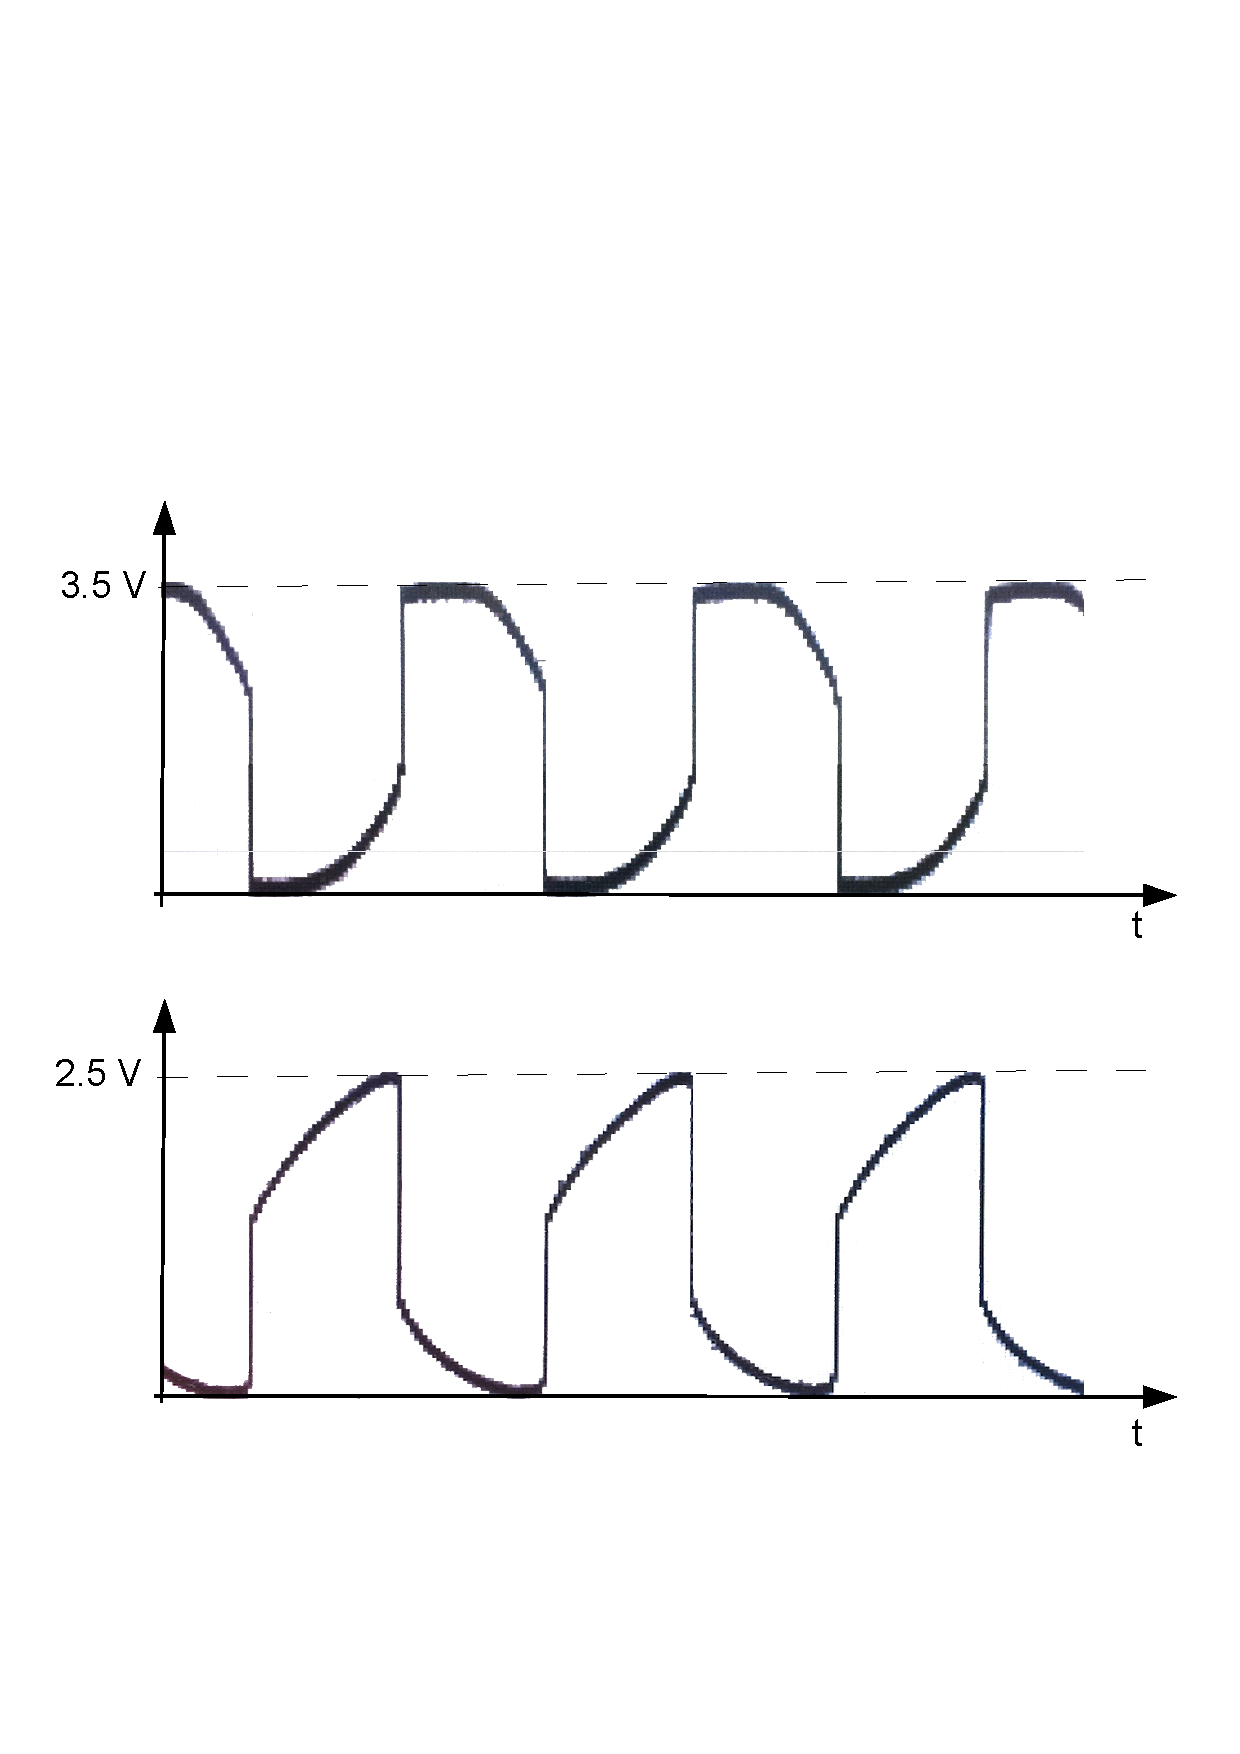
\includegraphics[trim=10mm 50mm 1mm 90mm, clip,
   width=\columnwidth]{img/am_timing.pdf}
   \caption{Timing diagram. Up: Voltage signal at $O1$; bottom: Voltage signal
   at $O2$.}
   \label{fig:am_timing}
\end{figure}


\begin{figure}
  \centering
   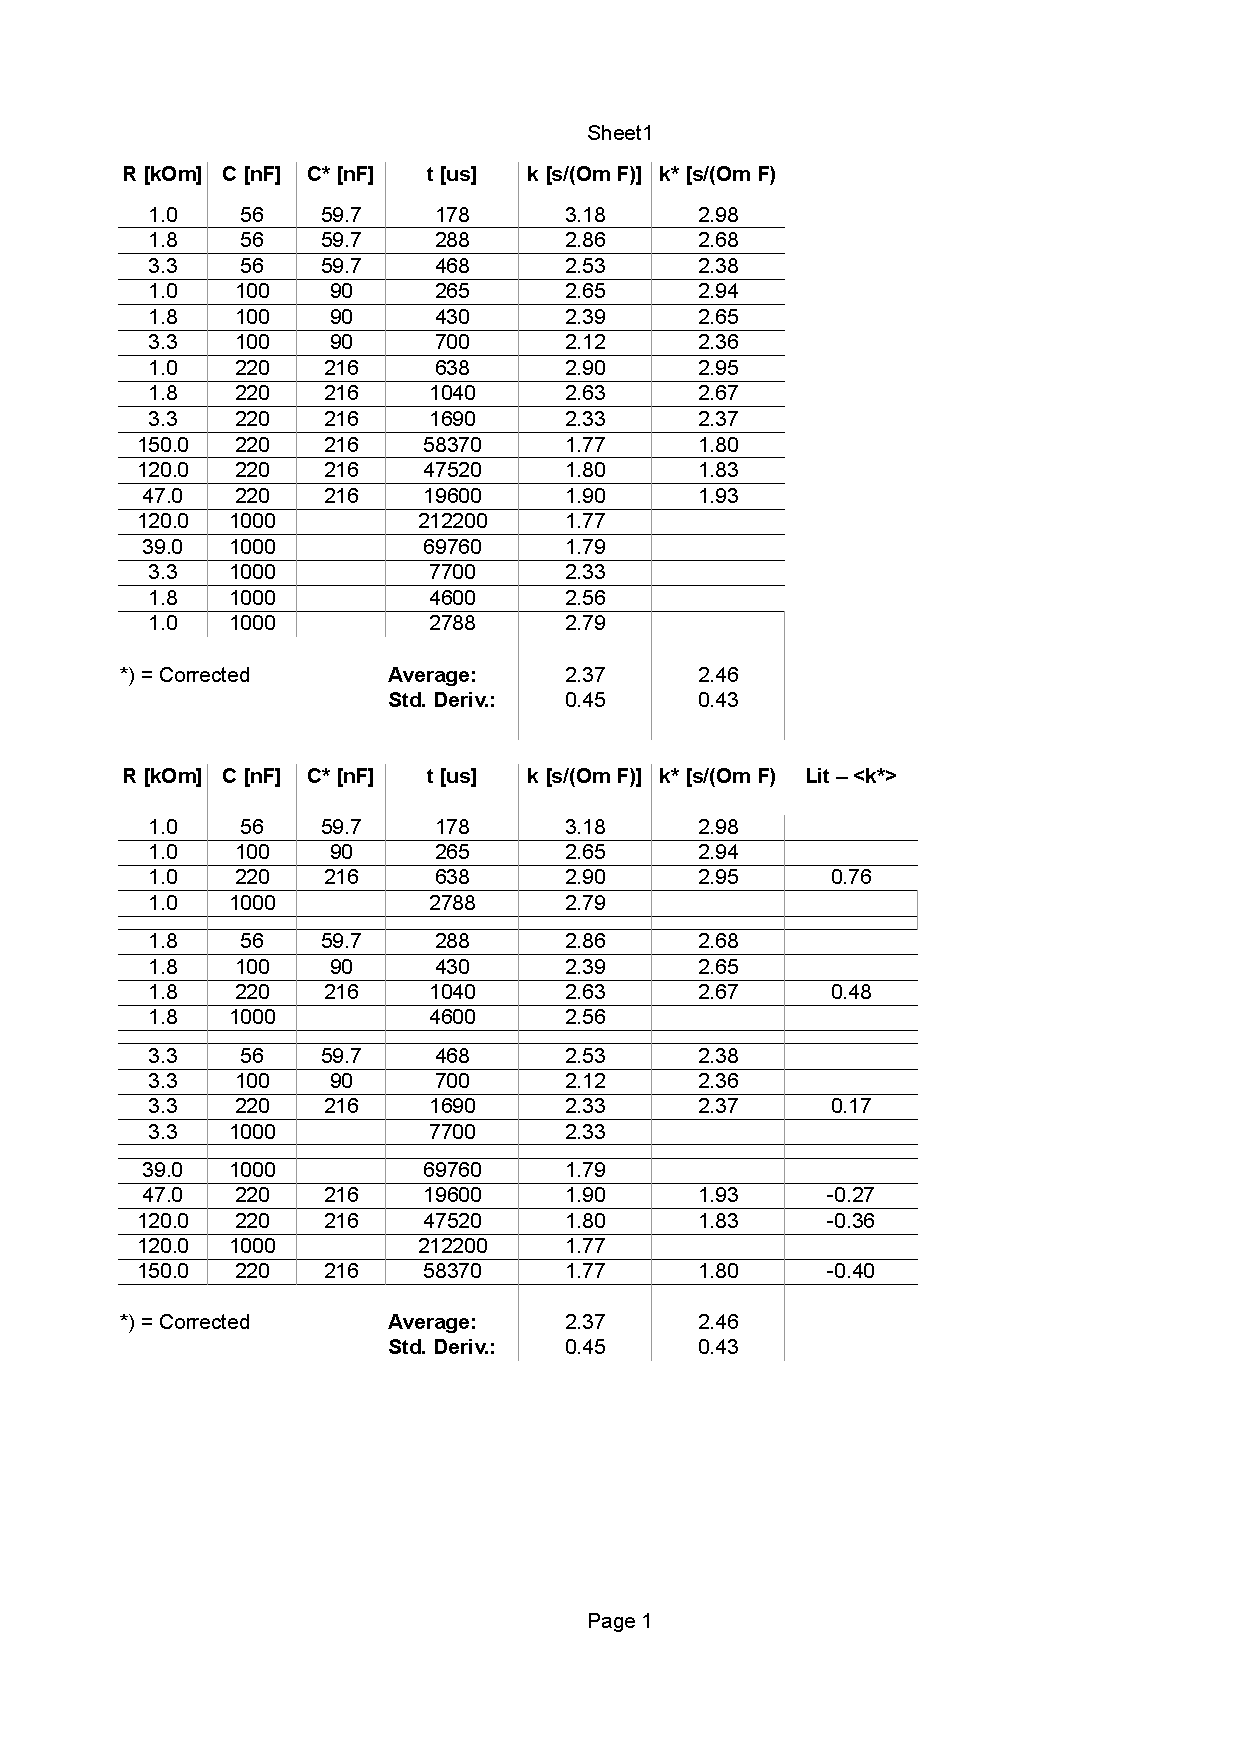
\includegraphics[trim=20mm 63mm 55mm 130mm, clip,
   width=\columnwidth]{results/am_data.pdf}
   \caption{Measurement of period time $t$ as function of resistance $R$ and
   capacity $C$.}
   \label{fig:am_result}
\end{figure}


The time diagram for the voltage at $O1$ and $O2$ is visualized in figure
\ref{fig:am_timing}. In table \ref{fig:am_result} different period times $t$ due 
to different choices of resistance $R$ and capacity $C$ are listed. The values
for the resistances and the capacities shown here are excluding a manufacturing
error of roughly up to $10\%$. Some of the capacities were more precise
measured and are listed in the $C*$ column.

\subsection{Analysis and Discussion}

The k-value is defined as

\begin{equation}
	k = \frac{t}{R \cdot C}
	\label{eq:k}
\end{equation}

where $t$ is the period time, $R$ is the resistance of the resistor
\em{R} and $C$ is the capacity of the capacitor \em{C}. Based on the
measurements, the k-values are computed in table \ref{fig:am_result} in the $k$
column. For the more precisely measured capacities $C*$, the k-value $k*$ was
computed using the $C*$ value.

As mentioned in \cite{book_dg}, the relation between $t$ and the other
quantities is given by

\begin{equation}
	t = 2~R~C~\ln(3) \approx 2.2~R~C
\end{equation}

which gives the value of $k$ using \ref{eq:k}

\begin{equation}
	k = 2~\ln(3) \approx 2.2
	\label{eq:k_lit}
\end{equation}

The average values of $k$ and $k*$ given in table \ref{fig:am_result} match very
well with the expected values for k. Using the standard derivation of the average as
an indicator for the uncertainty of the here measured $k$ and $k*$ values, the
literal value is within the range of average +- standard derivation. However,
the standard derivation is larger then 1/10 of the average value. This indicates
a high uncertainty.

\begin{figure}
  \centering
   \includegraphics[trim=50mm 90mm 45mm 125mm, clip,
   width=\columnwidth,page=2]{results/am_data.pdf}
   \caption{Measurement of period time $t$ as function of resistance $R$ and
   capacity $C$.}
   \label{fig:am_plot}
\end{figure}

The last column $Lit - \<k*\>$ holds the difference between the literature value
\ref{eq:k_lit} and the calculated $k*$ value and therefore a simple error
estimation between measurement and literature value. The error is calculated for
the same capacitor $C = 200\text{nF}$. A plot of these errors is shown in 
\ref{fig:am_plot}. The X-axis is plotted logarithmically. The shape of the curve
suggests a exponential relation between $R$ and the error. As the $k*$ values
are roughly the same for different choices of $C$, this might be an indication,
that the error is mostly related to the choice of the resistance. The reason for
this correspondence remained unclear to the author.

\subsection{Schlussfolgerung und Ausblick }

\section{Die Messmethode und der experimentelle Aufbau}

\section{Die Messergebnisse}

\begin{center}
\line(1,0){250}
\end{center}

\begin{thebibliography}{------}
\bibitem[BOOK]{book_dg}
	U. Tietze, C. Schenk
	{\em Halbleiter-Schaltungstechnik}.
	Springer, sechste, neue Überarbeitete und erweiterte Auflage (1983), pp
	176-177
\end{thebibliography}

\end{document}
